\documentclass{ctexart}
\usepackage[T1]{fontenc}
\usepackage[a4paper,top=3cm,bottom=3cm,left=1.75cm,right=1.75cm,marginparwidth=1.75cm]{geometry}
\usepackage{mathtools}
\usepackage{booktabs}
\usepackage{caption}
\usepackage{outlines}
\usepackage{amsthm}
\usepackage{graphicx}
\usepackage{minted}
\usepackage{float}
\usepackage{hyperref}
\usepackage[nameinlink]{cleveref}
\usepackage{algorithm}
\usepackage{algorithmicx}
\usepackage{algpseudocode}
\usepackage{chngcntr}
\usepackage{gbt7714}

\newcommand*{\fullref}[1]{\hyperref[{#1}]{\Cref*{#1} \nameref*{#1}}}
\renewcommand{\algorithmicrequire}{\textbf{Input:}}
\renewcommand{\algorithmicensure}{\textbf{Output:}}
\counterwithin{table}{section}
\counterwithin{table}{subsection}
\renewcommand{\tableautorefname}{表}
\crefname{equation}{方程}{方程}
\crefname{algorithm}{算法}{算法}
\crefname{lemma}{引理}{引理}
\crefname{table}{表}{表}
\crefname{figure}{图}{图}
\newtheorem{definition}{定义}[section]
\newtheorem{example}{例}[section]
\newtheorem{theorem}{定理}[section]
\newtheorem{lemma}{引理}[section]
\DeclarePairedDelimiter{\set}{\{}{\}}
\DeclarePairedDelimiter{\paren}{(}{)}
\graphicspath{ {./images/} }
\setmonofont{JetbrainsMono-Regular.ttf}
\newcommand{\fibheap}{\texttt{fibonacci heap }}
\newcommand{\fibnode}{\texttt{fibonacci heap node }}
\newcommand{\push}{\texttt{push }}
\newcommand{\pop}{\texttt{pop }}
\newcommand{\deckey}{\texttt{decrease key }}
\newcommand{\includedrawio}[2][]{
    \immediate\write18{/Applications/draw.io.app/Contents/MacOS/draw.io #2 --crop -x -o #2.pdf}
    \includegraphics[#1]{#2.pdf}
}

\ctexset{
    section = {
        titleformat = \centering\heiti\zihao{3},
        name = {,},
        aftertitle = \hspace{12pt},
    },
    subsection = {
        titleformat = \raggedright\heiti\zihao{4},
        name = {,},
        aftertitle = \hspace{6pt},
        indent = 2\ccwd
    },
    subsubsection = {
        titleformat = \raggedright\heiti\zihao{-4},
        name = {,},
        aftertitle = \hspace{3pt},
        indent = 2\ccwd
    },
    paragraph = {
        runin = false,
        indent = 2\ccwd
    },
    today = small,
    figurename = 图,
    contentsname = 目录,
    tablename = 表,
}

\begin{document}

\begin{titlepage}
    \centering
    \rule{\textwidth}{0pt}
    \vspace{0.3\textheight}
    
    {\zihao{2} \heiti 数据结构与算法 课程设计报告}
    
    \vspace{0.2\textheight}
    {
        \zihao{4}\selectfont \songti
        学~~~~~~号 \underline{\qquad\;19071125\;\qquad} \\
        姓~~~~~~名 \underline{\qquad~~卢雨轩~~\qquad} \\ 
        指导教师   \underline{\qquad~~杜永萍~~\qquad} \\
    }
    \vfill
    
    {\zihao{5} \songti \today}
    
    \vspace{0.25\textheight}
\end{titlepage}

% 目录
\tableofcontents
\clearpage

\section{需求分析}
\subsection{题目描述}
% \subsubsection{需求分析}

设飞机场有四条跑道,四条都可以用于起飞,其中三条用于正常着陆,第四条用于紧急着陆。要求为飞机安排对应的跑道在规定的时间起飞或降落。当飞机出现时,则根据飞机航班号,燃油储备量等,将飞机排入队列。

在机场发生的事件为:

\begin{outline}[enumerate]
\1 每单位时间最多有4架飞机进入起飞队列,最多有4架飞机进入着陆队列;
\1 每条跑道在一个单位时间内只允许一次起飞或降落;
\1 在每个单位时间中,任何一个着陆队列里机载燃油接近最低储备量的飞机必需给与高于其他飞机的优先级,进行降落。如果仅有一架飞机出现这种状况,则使用第4条跑道,如果多于1架(最多4架)飞机出现此状况,则也要使用其他跑道。条件是保证安全,不能在跑道上发生撞机,不能因燃油耗尽发生坠机,充分利用跑道资源。
\end{outline}

请设计程序系统模拟为各航班飞机安排跑道进行起飞或降落的管理模式。
\subsection{需求分析}
\begin{outline}
    \1 维护起飞、降落队列
    \1 维护紧急降落队列
    \1 每单位时间从队列中取出飞机,放入跑道
    \1 可视化飞机起飞、队列、航班时刻表
\end{outline}
\subsection{需求实现}
% \begin{outline}[enumerate]
\subsubsection{使用类似『多级反馈队列』算法的方式调度飞机。}

注意到:把飞机调度到跑到上,和操作系统中把进程调度到CPU的核心上,某种意义上是类似的。因此,我们可以使用类似『多级反馈队列』算法的方式来调度飞机。

令$W_i$为飞机$i$等待的时间,$fuel_i$为飞机$i$的剩余燃油量,$N_i$为飞机$i$的调度优先级(nice值),则我们可以给每个飞机计算一个当前优先级:

\begin{equation*}
    P_i = \frac{W_i}{F(i)} - 2 \times N_i
\end{equation*}

其中,$F(i)$为飞机$i$的燃油指数:

\begin{equation*}
    F(i) = \begin{cases}
        1 & \text{飞机要起飞} \\
        \frac{\exp(\mathrm{FuelFactor} \times (F_i - 20))}{\exp(\mathrm{FuelFactor} \times (F_i - 20)) + 1} & \text{飞机要降落} \\
    \end{cases}
\end{equation*}

下面,我们逐个分析以上的实现如何实现了每个需求:

\begin{outline}
    \1 维护起飞、降落队列:

        将起飞和队列的飞机放入优先队列中,通过以上的方式计算权重。
    \1 维护紧急降落队列

        由上述计算燃油指数的方式,我们可以得到:
        \2 当飞机要起飞时,燃油指数为1,单纯通过飞机的等待时间和调度优先级进行排序。
        \2 当飞机要降落且剩余燃油量大于20时,燃油指数是一个接近1的数,同样单纯通过飞机的等待时间和调度优先级调度。
        \2 当飞机要降落且剩余燃油量小于20时,燃油指数是一个接近0的数,飞机的优先级趋近于正无穷,一定在优先队列的前端。

        因此,通过以上方式就能保证紧急降落的飞机一定先出队,不需要单独维护紧急降落队列。
    \1 每单位时间从队列中取出飞机,放入跑道

        只需要每单位时间从队列中取出飞机,放入跑道。其中筛选出紧急着陆或起飞的飞机放入第四条跑道。

    \1 可视化飞机起飞、队列、航班时刻表

        读取队列内信息渲染即可。
\end{outline}

可以看到,上述实现满足题目描述中的需求。

\subsection{开发环境}

考虑到需要要可视化的信息较多,且渲染较为复杂,课设使用\texttt{TypeScript}语言开发,并在浏览器内运行。

\subsubsection{界面渲染}

渲染图形界面较为复杂,很难抽象为\texttt{HTML},因此项目使用\texttt{PIXI.js}图形开发框架,通过\texttt{WebGL}或\texttt{Canvas API} 绘制到\texttt{canvas}中。这样实现尽可能的兼容了更多平台,还可以使用GPU加速渲染界面。

\subsection{界面设计}

\begin{figure}[H]
    \centering
    \includedrawio[width=\textwidth]{user-interface.drawio}
    \caption{机场管理系统 界面设计}
\end{figure}

\section{数据结构设计}

\subsection{队列实现}

使用斐波那契堆(Fibonacci heap)维护起飞、降落队列。数据结构设计如下:

\begin{figure}[H]
    \centering
    \includedrawio[width=.7\textwidth]{fibonacci-heap.drawio}
    \caption{斐波那契堆 结构}
\end{figure}

\subsection{其他数据结构}
下面给出其他数据结构的定义。

\subsubsection{飞机}
\begin{minted}[linenos]{typescript}
class Plane {
    name: string;
    type: 'takeoff' | 'landing';
    time: moment.Moment;
    fuel: number; // will be ignored during takeoff.
    nice: number;
    waitTime: number;
    heapNode: FibHeapNode;
    status: 'waiting' | 'queueing' | 'served' | 'crashed';
    sprite: PIXI.Container;

    constructor(name: string,
        type: 'takeoff' | 'landing',
        time: moment.Moment,
        fuel: number,
        nice: number)

    getSprite(): PIXI.Container

    priority(): number

    toString(): string
}
\end{minted}
\subsubsection{机场}
\begin{minted}[linenos]{typescript}
class Airport {
    planes: Array<Plane>;
    queue: FibHeap;
    takeoffLoad: number;
    landingLoad: number;
    currentTime: moment.Moment;
    planesOutQueue: Array<Plane>;
    servedCount: number;
    crashedPlanes: Array<Plane>;

    constructor()
    addPlane(options: addPlaneOption)

    interval(debug: boolean = false)
}
\end{minted}
\subsection{模块功能描述}
\begin{minted}[]{text}
├── assets              资源文件
│   ├── airport.png
│   ├── home.png
│   ├── load-hover.png
│   ├── load.png
│   ├── novem__.woff
│   └── plane.png
├── import-png.d.ts
├── index.ts            主程序代码
├── lib
│   ├── airport.ts      机场数据结构和调度算法
│   ├── config.ts       参数设置
│   ├── fibonacci.ts    fibonacci heap
│   ├── plane.ts        飞机数据结构和优先级计算
│   └── tree.ts         fibonacci heap visualize
├── stages              界面渲染相关
│   ├── loadStage.ts    加载界面
│   └── main.ts         主程序界面
├── style
│   └── main.scss       代码格式控制
├── test.ts
└── utils
    └── time.ts         虚拟时间戳
\end{minted}
\section{详细设计}
\subsection{优先队列实现}
由于项目设计把两类飞机放入同一个队列中,并有大量的更改权重操作,如果使用朴素的二叉堆,每个时间周期的操作的时间复杂度会为$O(n\log(n))$。因此,在有大量更新权重且只有少量\texttt{push}、\texttt{pop}操作时,应该采用\texttt{fibonacci heap}。

\subsubsection{\fibheap 简介}
\fibheap 是一种可合并堆,可以支持高效的\deckey 操作。与二叉堆的对比详见\fullref{table:fib-and-binary-heap}。

\begin{table}[htp]
    \centering
    \begin{tabular}{ccc}
        \toprule
        操作 & \fibheap & 二叉堆 \\
        \midrule
        MAKE-HEAP   & $O(1)$    & $O(1)$ \\
        INSERT      & $O(\lg n)$& $O(\lg n)$ \\
        MINIMUM     & $O(1)$    & $O(1)$ \\
        EXTRACT-MIN & $O(\lg n)$& $O(\lg n)$ \\
        UNION       & $O(1)$    & $O(n)$ \\
        DECREASE-KEY & $O(1)$   & $O(\lg n)$ \\
        DELETE      & $O(\lg n)$& $O(\lg n)$ \\
        \bottomrule
    \end{tabular}
    \caption{\fibheap 与二叉堆对比}
    \label{table:fib-and-binary-heap}
\end{table}
\subsubsection{\fibheap 结构}
一个 \fibheap 是一个具有最小堆性质的有根树的集合(森林),也就是说,每个结点的关键字均大于或等于他父结点的关键字。我们维护每个节点的父亲、孩子(双向循环链表)、度数、标记(某结点自从上一次成为另一个结点的孩子后,是否失去孩子)。同时,我们维护整个堆的最小结点(也就是森林中的树的根节点中最小的)。如果\fibheap 是空的,那么 min 为NULL。

\subsubsection{势函数}
我们将要使用势方法分析\fibheap 的时间复杂度。对于一个给定的\fibheap H,用$t(H)$表示H根链表中节点的数目,用$m(H)$中表示h中已标记的节点的数目,然后定义\fibheap H的势函数如下:

\begin{equation*}
    \Phi(H) = t(H) + 2m(H)
\end{equation*}

\subsubsection{最大度数}

可以证明,在一个有$n$个结点的\fibheap 中,任何结点的最大度数的上界$D(n) = \lg_{(1 + \sqrt{5}) / 2}(n)$

\subsubsection{\fibheap 的操作}
\paragraph{MAKE-HEAP}
\begin{algorithm}
    \caption{MAKE-HEAP}
    \begin{algorithmic}[1]
        \Ensure \fibheap H
        \State $H.min \gets NIL$
        \State $H.n \gets 0$
    \end{algorithmic}
\end{algorithm}
不难看出,时间复杂度为$O(1)$。

\paragraph{INSERT-NODE}
\begin{algorithm}
    \caption{INSERT-NODE}
    \begin{algorithmic}[1]
        \Require \fibheap H, \fibnode x
        % \Ensure \fibheap H
        \State $x.degree \gets 0$
        \State $x.p \gets NIL$
        \State $x.child \gets NIL$
        \State $x.marl \gets False$
        \If{$H.min = NIL$}
            \State Create a root list of H containing just x.
            \State $H.min \gets x$
        \Else
            \State insert x into H's root list.
            \If{$x.key < H.min.key$}
                \State $H.min \gets x$
            \EndIf
        \EndIf
        \State $H.n \gets H.n + 1$
    \end{algorithmic}
\end{algorithm}
在插入结点的时候,我们直接将结点插入到H的root list中。操作的时间复杂度显然是$O(1)$,势函数的变化量为

\begin{align*}
    \Delta \Phi &= \Phi(H') - \Phi(H) \\
                & = t(H) + 1 + 2 m(H) - (t(H) + 2m(H)) \\
                & =1
\end{align*}

所以,实际平均代价为$O(1) +  1 = O(1)$。

\paragraph{MINIMUM}

显然,获取最小元素的时间复杂度为$O(1)$。

\paragraph{UNION}

合并两个堆,只需要将他们的root list合并,维护min,并更新堆大小n。势函数变化量为

\begin{align*}
    \Delta \Phi &= \Phi(H) - \Phi(H_1) - \Phi(H_2) \\
                & = t(H) + 2 m(H) - (t(H_1) + 2m(H_1))  - (t(H_2) + 2m(H_2))\\
                & =0
\end{align*}

显然,时间复杂度为$O(1)$

\paragraph{EXTRACT-MIN}
\begin{algorithm}
    \caption{EXTRACT-MIN}
    \begin{algorithmic}[1]
        \Require \fibheap H
        \State $z \gets H.min$
        \If{$z \ne NIL$}
            \For{child $x$ of $z$}
                \State insert $x$ into H's root list
                \State $x.p \gets NIL$
            \EndFor
            \State remove $z$ from H's root list
            \If{H's root list is empty}
                \State $H.min \gets NIL$ \Comment{now H is empty}
            \Else
                \State $H.min \gets $ next child of Z's root list \Comment{For now we set a random node as min}
                \State CONSOLIDATE(H) \Comment{Consolidate nodes if needed}
            \EndIf
        \EndIf
    \end{algorithmic}
\end{algorithm}

在移除最小结点的时候,我们首先将他的所有孩子插入到root list中,然后调用CONSOLIDATE合并具有相同度数的结点,保证每个度数至多只有1个结点在root list 中。

\begin{algorithm}[htp]
    \caption{CONSOLIDATE}
    \begin{algorithmic}[1]
        \Require \fibheap H
        \State Let $A$ be an empty array with length $D(H.n)$.
        \For{each child $w$ of H's root list}
            \State $x \gets w$
            \State $d \gets x.degree$
            \While{$A[d] \ne NIL$} \Comment{Consolidate nodes with same degree}
                \State $y \gets A[d]$
                \If{$x.key > y.key$}
                    \State swap $x$ and $y$
                \EndIf
                \State remove $y$ from H's root list
                \State make $y$ a child of x, incrementing $x$'s degree
                \State $y.mark \gets False$ \Comment{$y$ becomes other node's child, clear it's mark}
                \State $A[d] \gets NIL$ \Comment{$A[d]$ is removed from root list}
                \State $d \gets d + 1$
            \EndWhile
            \State $A[d] \gets x$ \Comment{now, there arn't node with degree same with x.}
        \EndFor
        \State $H.min \gets NIL$
        \For{$i \gets 0$ to $D(H.n)$}
            \If{$A[i] \ne NIL$}
                \If{$H.min = NIL$}
                    \State Create a root list of H containing just $A[i]$.
                    \State $H.min \gets A[i]$
                \Else
                    \State insert A[i] into H's root list.
                    \If{$A[i].key < H.min.key$}
                        \State $H.min \gets A[i]$
                    \EndIf
                \EndIf
            \EndIf
        \EndFor
    \end{algorithmic}
\end{algorithm}
下面计算EXTRACT-MIN操作的时间复杂度。首先,单次运行EXTRACT-MIN的时间复杂度显然为$O(D(n))$。CONSOLIDATE的第19 -- 31行的工作需要的时间代价为$O(D(n))$。第2 -- 17行的时间复杂度为根链表的元素数量,也就是$O(t(H) + D(H) - 1)$,因此运行EXTRACT-MIN的时间复杂度为$O(D(n) + t(H))$。势函数变化量为:

\begin{align*}
    \Delta \Phi & = ((D(n) + 1 ) + 2m(H)) - (t(H) + 2m(H)) \\
                & = D(n) + 1 - t(H)
\end{align*}

因此,总的时间复杂度为$O(D(n) + t(H)) + \Delta \Phi = O(D(n))$。后面可以证明,$D(n) = O(\lg n)$,因此EXTRACT-MIN的摊还时间复杂度为$O(\lg n)$。

\paragraph{DECREASE-KEY}
\begin{algorithm}
    \caption{DECREASE-KEY}
    \begin{algorithmic}[1]
        \Require \fibheap H, \fibnode x, new key k
        \If{$k \ge x.key$}
            \State \textbf{error} \Comment{We can only decrease key}
        \EndIf
        \State $x.key \gets k$
        \State $y \gets x.p$
        \If{$y \ne NIL$ and $x.key < y.key$}
            \State CUT(H, x, y)
            \State CASCADING-CUT(H, y)
        \EndIf
        \If{$x.key < H.min.key$}
            \State $H.min \gets x$
        \EndIf
    \end{algorithmic}
\end{algorithm}
\begin{algorithm}
    \caption{CUT}
    \begin{algorithmic}[1]
        \Require \fibheap H, \fibnode x, y
        \State remove x from y's child list, decrementing y's degree.
        \State add x to the root list of H
        \State $x.p \gets NIL$
        \State $x.mark \gets FALSE$
    \end{algorithmic}
\end{algorithm}
\begin{algorithm}
    \caption{CASCADING-CUT}
    \begin{algorithmic}[1]
        \Require \fibheap H, \fibnode y
        \State $z \gets y.p$
        \If{$z \ne NIL$}
            \If{$y.mark = FALSE$}
                \State $y.mark \gets TRUE$
            \Else
                \State CUT(H, y, z)
                \State CASCADING-CUT(H, z)
            \EndIf
        \EndIf
    \end{algorithmic}
\end{algorithm}
首先我们把x的key减小。接着,如果x是根节点或者新的key没有大于x的父亲的key,则我们不需要做任何操作。否则,我们需要做很多操作。

首先,我们切断x。CUT过程将x从y的孩子中取出,使其成为根节点。

接着,我们通过mark来维护我们的时间复杂度。如果某个结点在成为别的孩子后已经失去一个孩子,那么此时它的mark应为TRUE,我们将它继续切断。我们一直沿着树递归向上进行CASCADING-CUT,直到某个结点的mark为FALSE或遇到根节点。

下面我们进行复杂度分析。首先分析它的实际代价。DECREASE-KEY过程需要$O(1)$的时间,还需要加上调用CASCADING-CUT的次数,我们设它为$c$。这样,总的实际运行时间就是$O(c)$。

接下来分析势函数的变化。
\begin{align*}
    \Delta \Phi &= ((t(H) + c) + 2(m(H) - c + 2)) - (t(H) + 2m(H)) \\
    &= 4 - c
\end{align*}
因此摊还时间复杂度为
\begin{equation*}
    O(c) + 4 - c = O(1)
\end{equation*}

\paragraph{总结}
可以看到,\fibheap 可以在$O(1)$时间内进行DECREASE-KEY操作,十分适合本项目这样,有大量DECREASE-KEY但是有较少的POP和PUSH操作的应用情景。

\subsubsection{最大度数的界}
上述复杂度分析过程中,我们一直假设$D(n) = O(\lg n)$。下面我们给出证明。

\begin{lemma}
    \label{lemma:1}
    设x是\fibheap 中的任意结点,并假设$x.degree = k$。设$y_1, y_2, \dots, y_n$为x的孩子,并按照先后顺序排列,则$y_1.degree \ge 0$,且当$i \ge 2$时$y_i.degree \ge i - 2$。
\end{lemma}
\begin{proof}
    显然,$y_1.degree \ge 0$。对于$i \ge 2$,当$y_i$进入x时,一定有$x.degree \ge i - 1$。此时,一定也有$y.degree \ge i - 1$(因为当且仅当$y.degree = x.degree$时,会执行CONSOLIDATE操作,将$y_i$放到x的子树中)。

    在这之后,由CUT操作中的mark属性保证了$y_i$不会连续是去两个孩子(否则就会被CASCADING-CUT,进入root list)。

    综上,$y.degree \ge i - 2$。
\end{proof}
\begin{lemma}
    \label{lemma:2}
    设x是\fibheap 中的任意结点,并设$k = x.degree$,则有$size(x) \ge F_{k+2} \ge \phi^k$,其中$\phi = (1 + \sqrt{5}) / 2$,$F_i$为fibonacci数列的第i项。
\end{lemma}
\begin{proof}
    设$s_k$为\fibheap 中度数为$k$的结点的最小可能size。显然,$s_0 = 1$,$s_1 = 2$,$size(x) \ge s_k$,且$s_k$随着k单调递增。

    设$y_1, y_2, \dots, y_n$为x的孩子,并按照先后顺序排列。则有:
    \begin{equation*}
        size(x) \ge s_k \ge 2 + \sum_{i = 2}^{k}s_{y_i}.degree \ge 2 + \sum_{i=2}^{k}s_{i-2}
    \end{equation*}
    其中最后一步由\fullref{lemma:1}得到。

    下面我们使用数学归纳法。首先,我们有$s_0 = 1$,$s_1 = 2$,因此$s_i \ge F_{i + 2}$在$i \le 1$时成立。
    \begin{align*}
        s_k & \ge 2 + \sum_{i=2}^{k}s_{i-2} \ge 2 + \sum_{i=2}^{k}F_i \\
            & = 1 + \sum_{i=0}^{k}F_i \\
            & = F_{k+2} \\
            & \ge \phi^k \qedhere
    \end{align*}
\end{proof}
\begin{theorem}
    一个n个结点的\fibheap 中任意结点的最大度数$D(n)$为$O(\lg n)$。
\end{theorem}
\begin{proof}
    设x是\fibheap 中的任意结点,并有$k = x.degree$。依据 \fullref{lemma:2},有$n \ge size(x) \ge \phi^k$。取以$\phi$为底的对数,得到$k \le \log_\phi n$。

    所以,任意结点的最大度数$D(n)$为$O(\lg n)$。\footnote{上述证明过程参考了算法导论} \cite{man_ping_2013}

\end{proof}
\subsubsection{总结}
综上所述,\fibheap 可以在$O(1)$时间内实现DECREASE-KEY,并在$O(\lg n)$时间内完成EXTRACT-MIN,十分适合我们的需求。

与传统的二叉堆实现对比,将每次操作的时间复杂度从$O(n \lg n)$降低到$O(n)$。
\subsection{机场调度实现}
每单位时间进行如下操作(见 \fullref{algo:airport-schedule})。首先我们更新整个机场的起飞、降落的负载,然后更新队列中等待的飞机的负载情况并更新其优先级。接着,我们从队列中取出3个飞机。如果3个飞机中有起飞或者紧急降落的飞机,我们则可以把他安排到第四个跑道,然后任意取出一个飞机放入剩余的跑到。如果不存在起飞或紧急降落的飞机,我们则需要寻找一个飞机放入第四个跑道。对于这种情况,我们遍历整个堆中的所有飞机,判断是否可以放入第四个跑道。
\begin{algorithm}
    \caption{机场调度实现}
    \label{algo:airport-schedule}
    \begin{algorithmic}[1]
        \State $L_t \gets LOAD\_FACTOR \times L_t + (1 - LOAD\_FACTOR) \times $ count of takeoff planes in queue.
        \State $L_l \gets LOAD\_FACTOR \times L_l + (1 - LOAD\_FACTOR) \times $ count of landing planes in queue.
        \For{plane p in queue}
            \State add p's wait time with load
            \State decrease p's fuel if landing
            \If{$p.fuel \le 0$}
                \State add p to crashed list
                \State remove p from heap
            \EndIf
            \State DECREASE-KEY(p, p.priority())
        \EndFor
        \For{plane p to be add into queue}
            \State add p into heap
        \EndFor
        \State $E \gets FALSE$
        \For{$i \gets $ 0 to $2$}
            \State pop a plane from heap
            \If{this plane is taking off or emgergency}
                \State $E \gets TRUE$
            \EndIf
        \EndFor
        \If{not $E$} \Comment{we havn't got a plane for lane 4}
            \While{not E or heap not empty}
                \State pop a plane from heap
                \If{this plane is takeoff or emergency}
                    \State \textbf{break}
                \EndIf
            \EndWhile
            \State push pop-ed plane into heap
        \Else
            \State pop a plane from heap
            \Comment{We have a plane for lane 4 now, so any plane will do.}
        \EndIf
        \State record served plane, update served count
    \end{algorithmic}
\end{algorithm}
\subsection{渲染实现}
为了实现流畅的渲染和计算,本项目分离逻辑帧与渲染帧,并提供调整时钟速率功能。在每个时间周期,首先进行一个或多个逻辑帧(与时钟速率有关),完成飞机状态、位置的运算,接下来进行一个渲染帧,完成跑道、飞机起飞动画、航班时刻表和\fibheap 的可视化渲染。

\section{测试}

项目使用多组数据进行了不同的测试。

\subsection{真实航班数据}
项目爬取了北京大兴国际机场某天的航班时刻表,并进行了测试。可以发现,项目可以正确运行、安排跑道、获取飞机的航空公司并渲染对应的尾翼图标(见\fullref{fig:airport-schedule-real-data})。

\begin{figure}[htp]
    \centering
    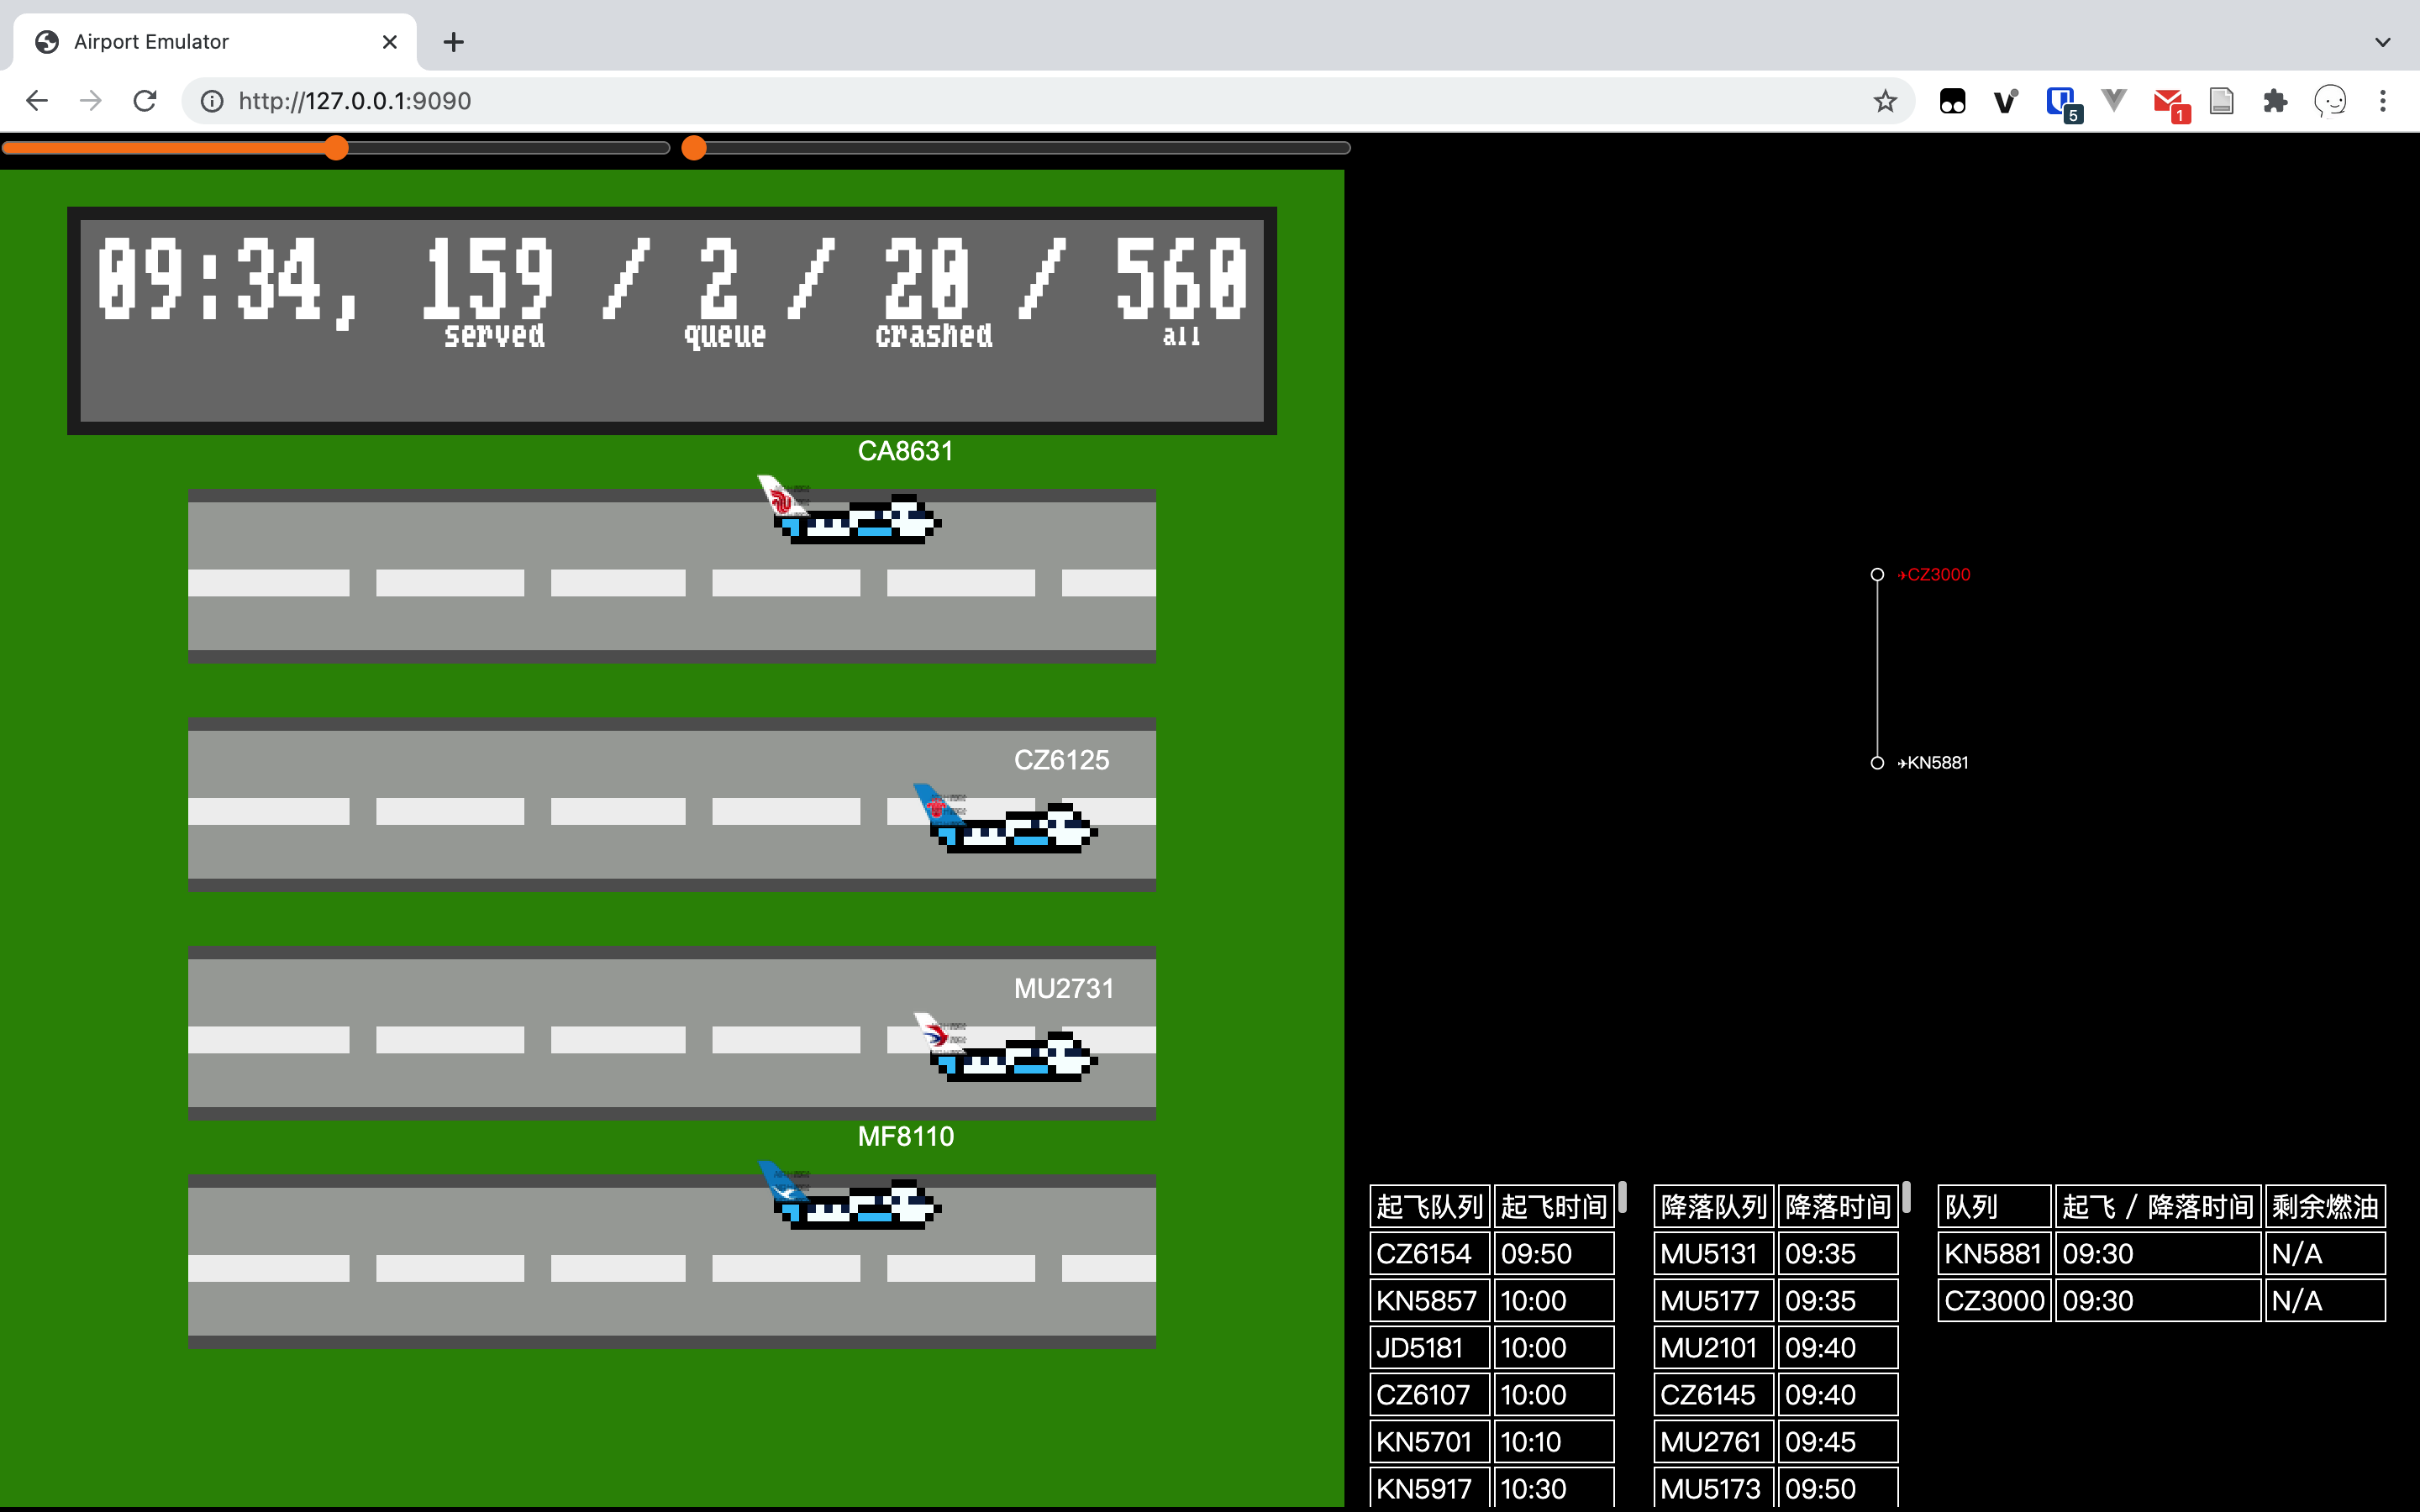
\includegraphics[width=0.9\textwidth]{images/test-1}
    \caption{真实航班数据 运行结果}
    \label{fig:airport-schedule-real-data}
\end{figure}

\subsection{格式错误数据}
项目能正确识别格式错误的数据,并提示用户格式非法(见\fullref{fig:test-illegal-input})

\begin{figure}[htp]
    \centering
    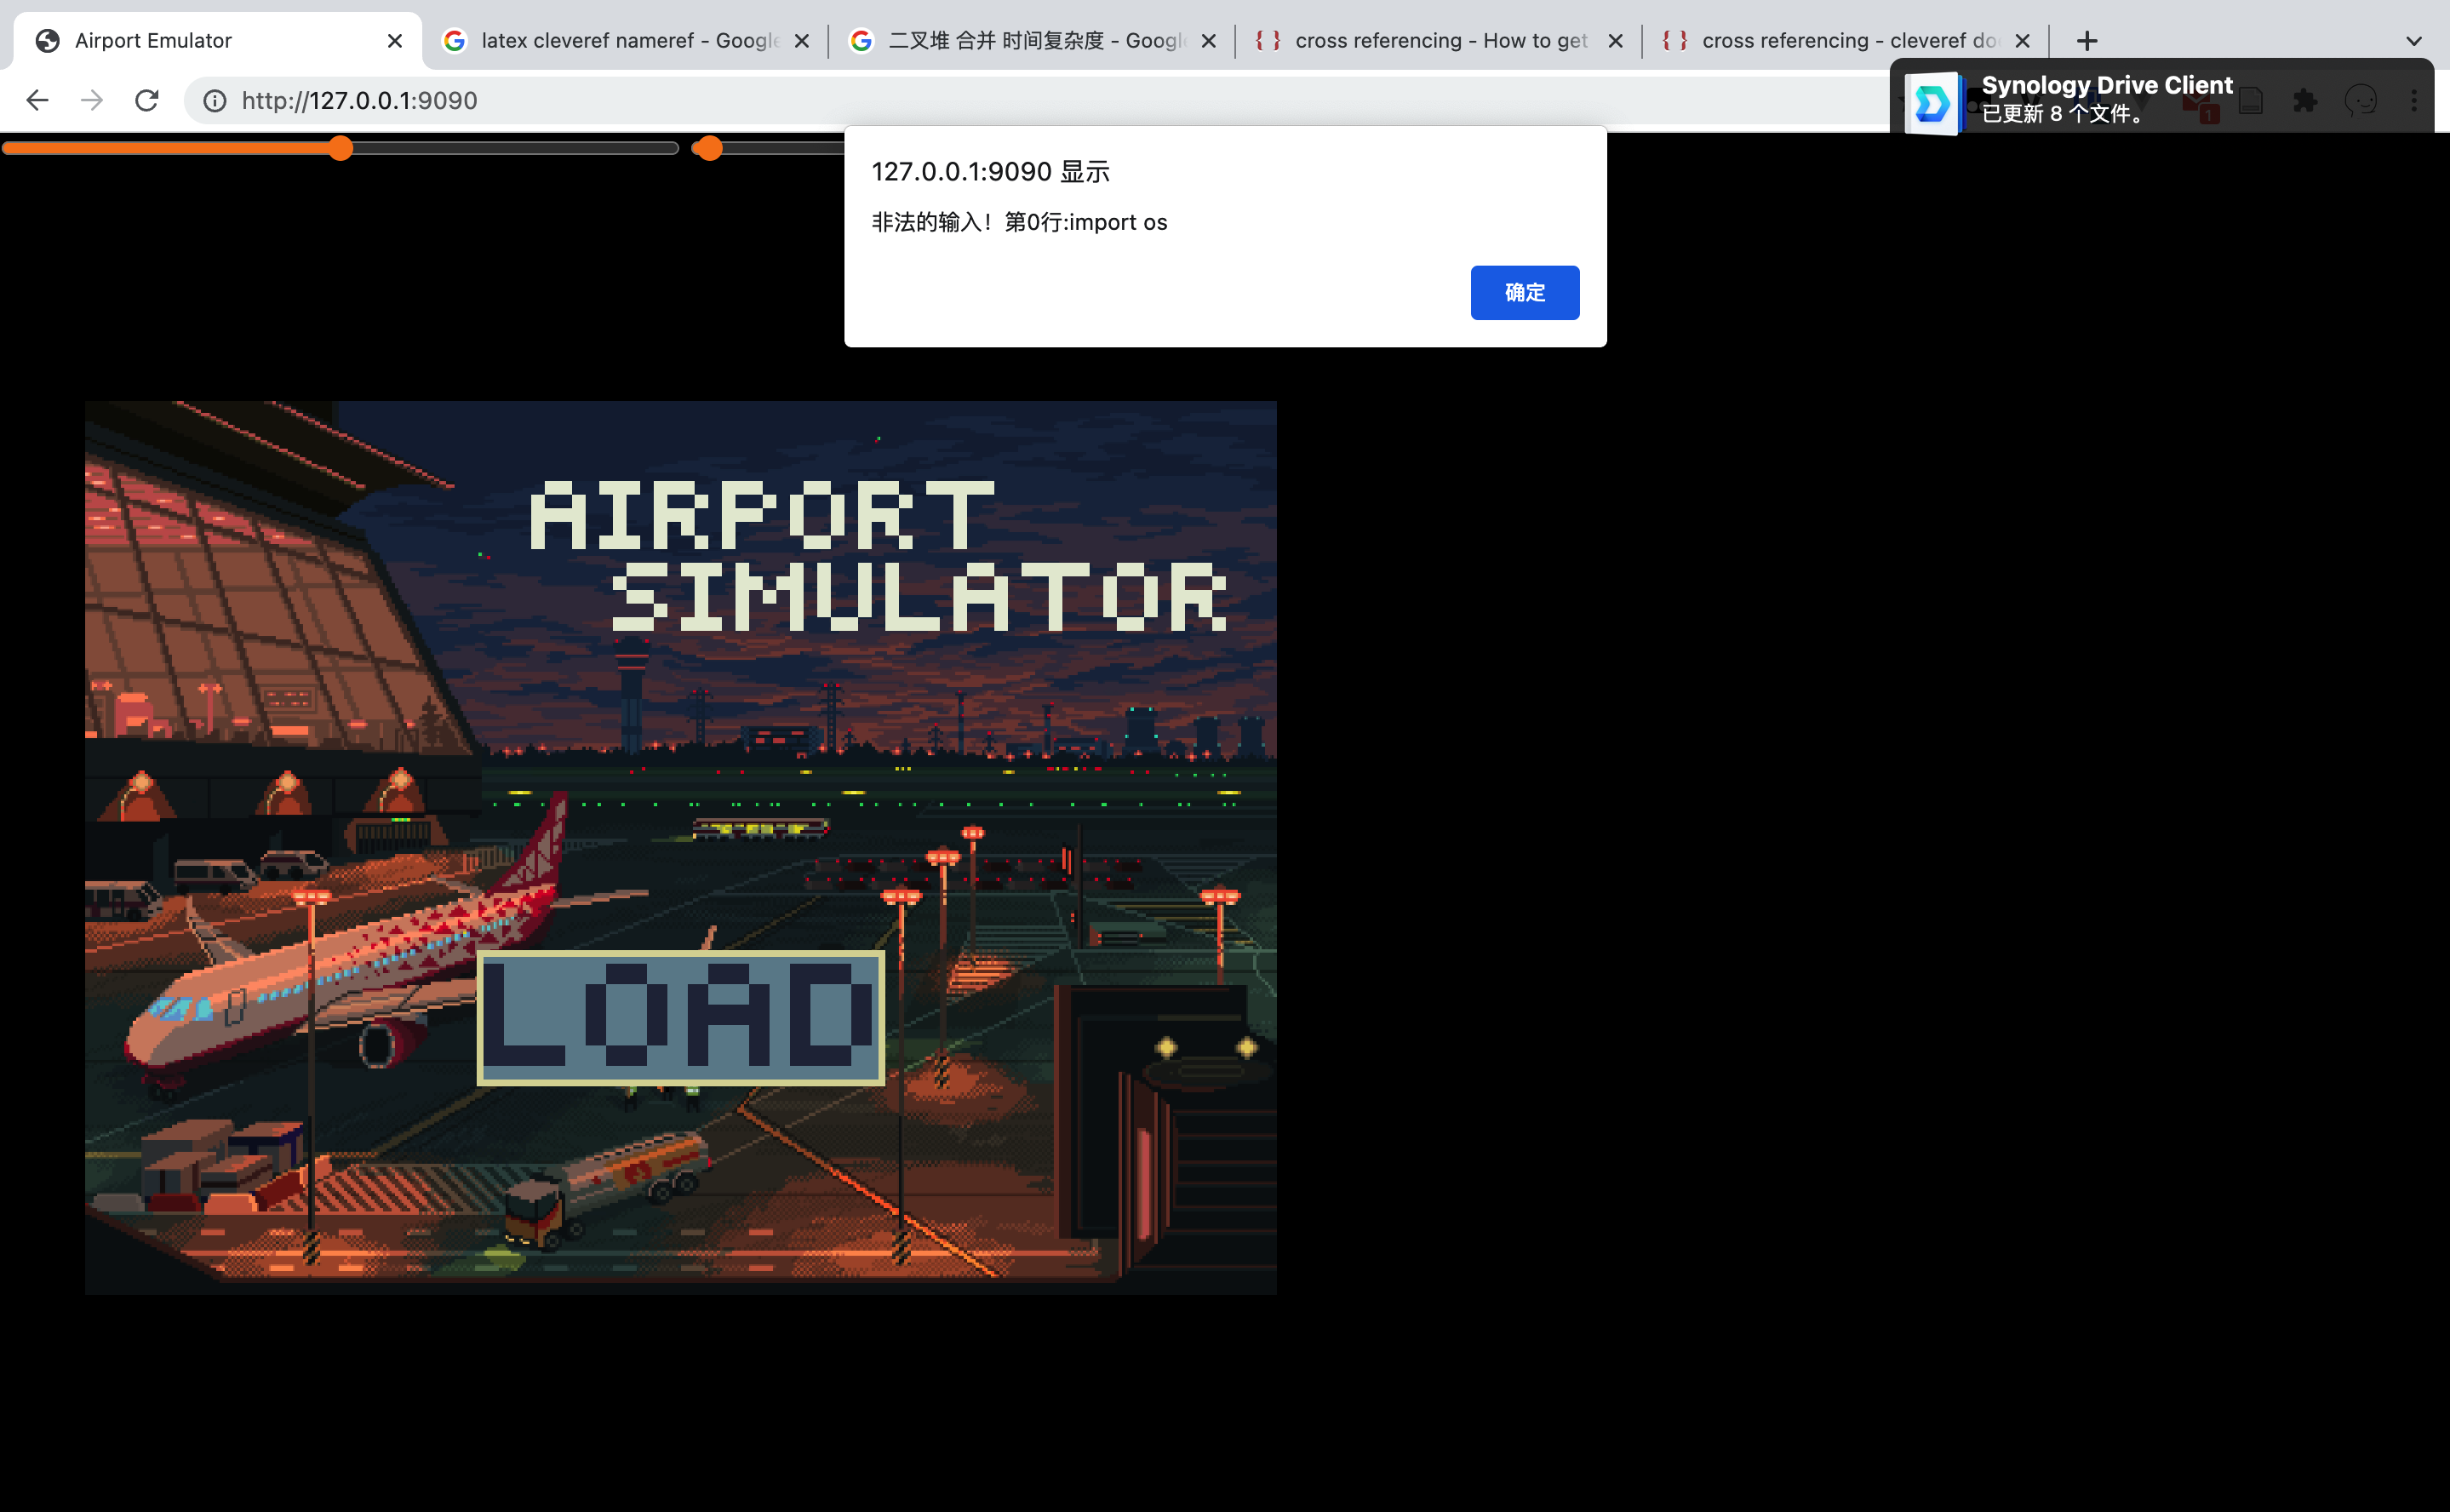
\includegraphics[width=0.9\textwidth]{images/test-wrong}
    \caption{非法输入\quad 运行结果}
    \label{fig:test-illegal-input}
\end{figure}

\clearpage 

\subsection{极端情况数据}
项目可以正确处理飞机数量极多、不得不坠机的数据。对此,我们构造了一组必定会有飞机坠毁的数据。可以看到,最开始飞机没有使用紧急降落跑道,燃油量也可以正确计算(\fullref{fig:test-crash-1})。稍后,等到有飞机的燃油量小于10时,第四条跑道被占用(\fullref{fig:test-crash-2})。最后,当飞机的燃油量小于0时,飞机被从队列中移除,并增加了坠毁计数器(\fullref{fig:test-crash-3})。

\begin{figure}[htp]
    \centering
    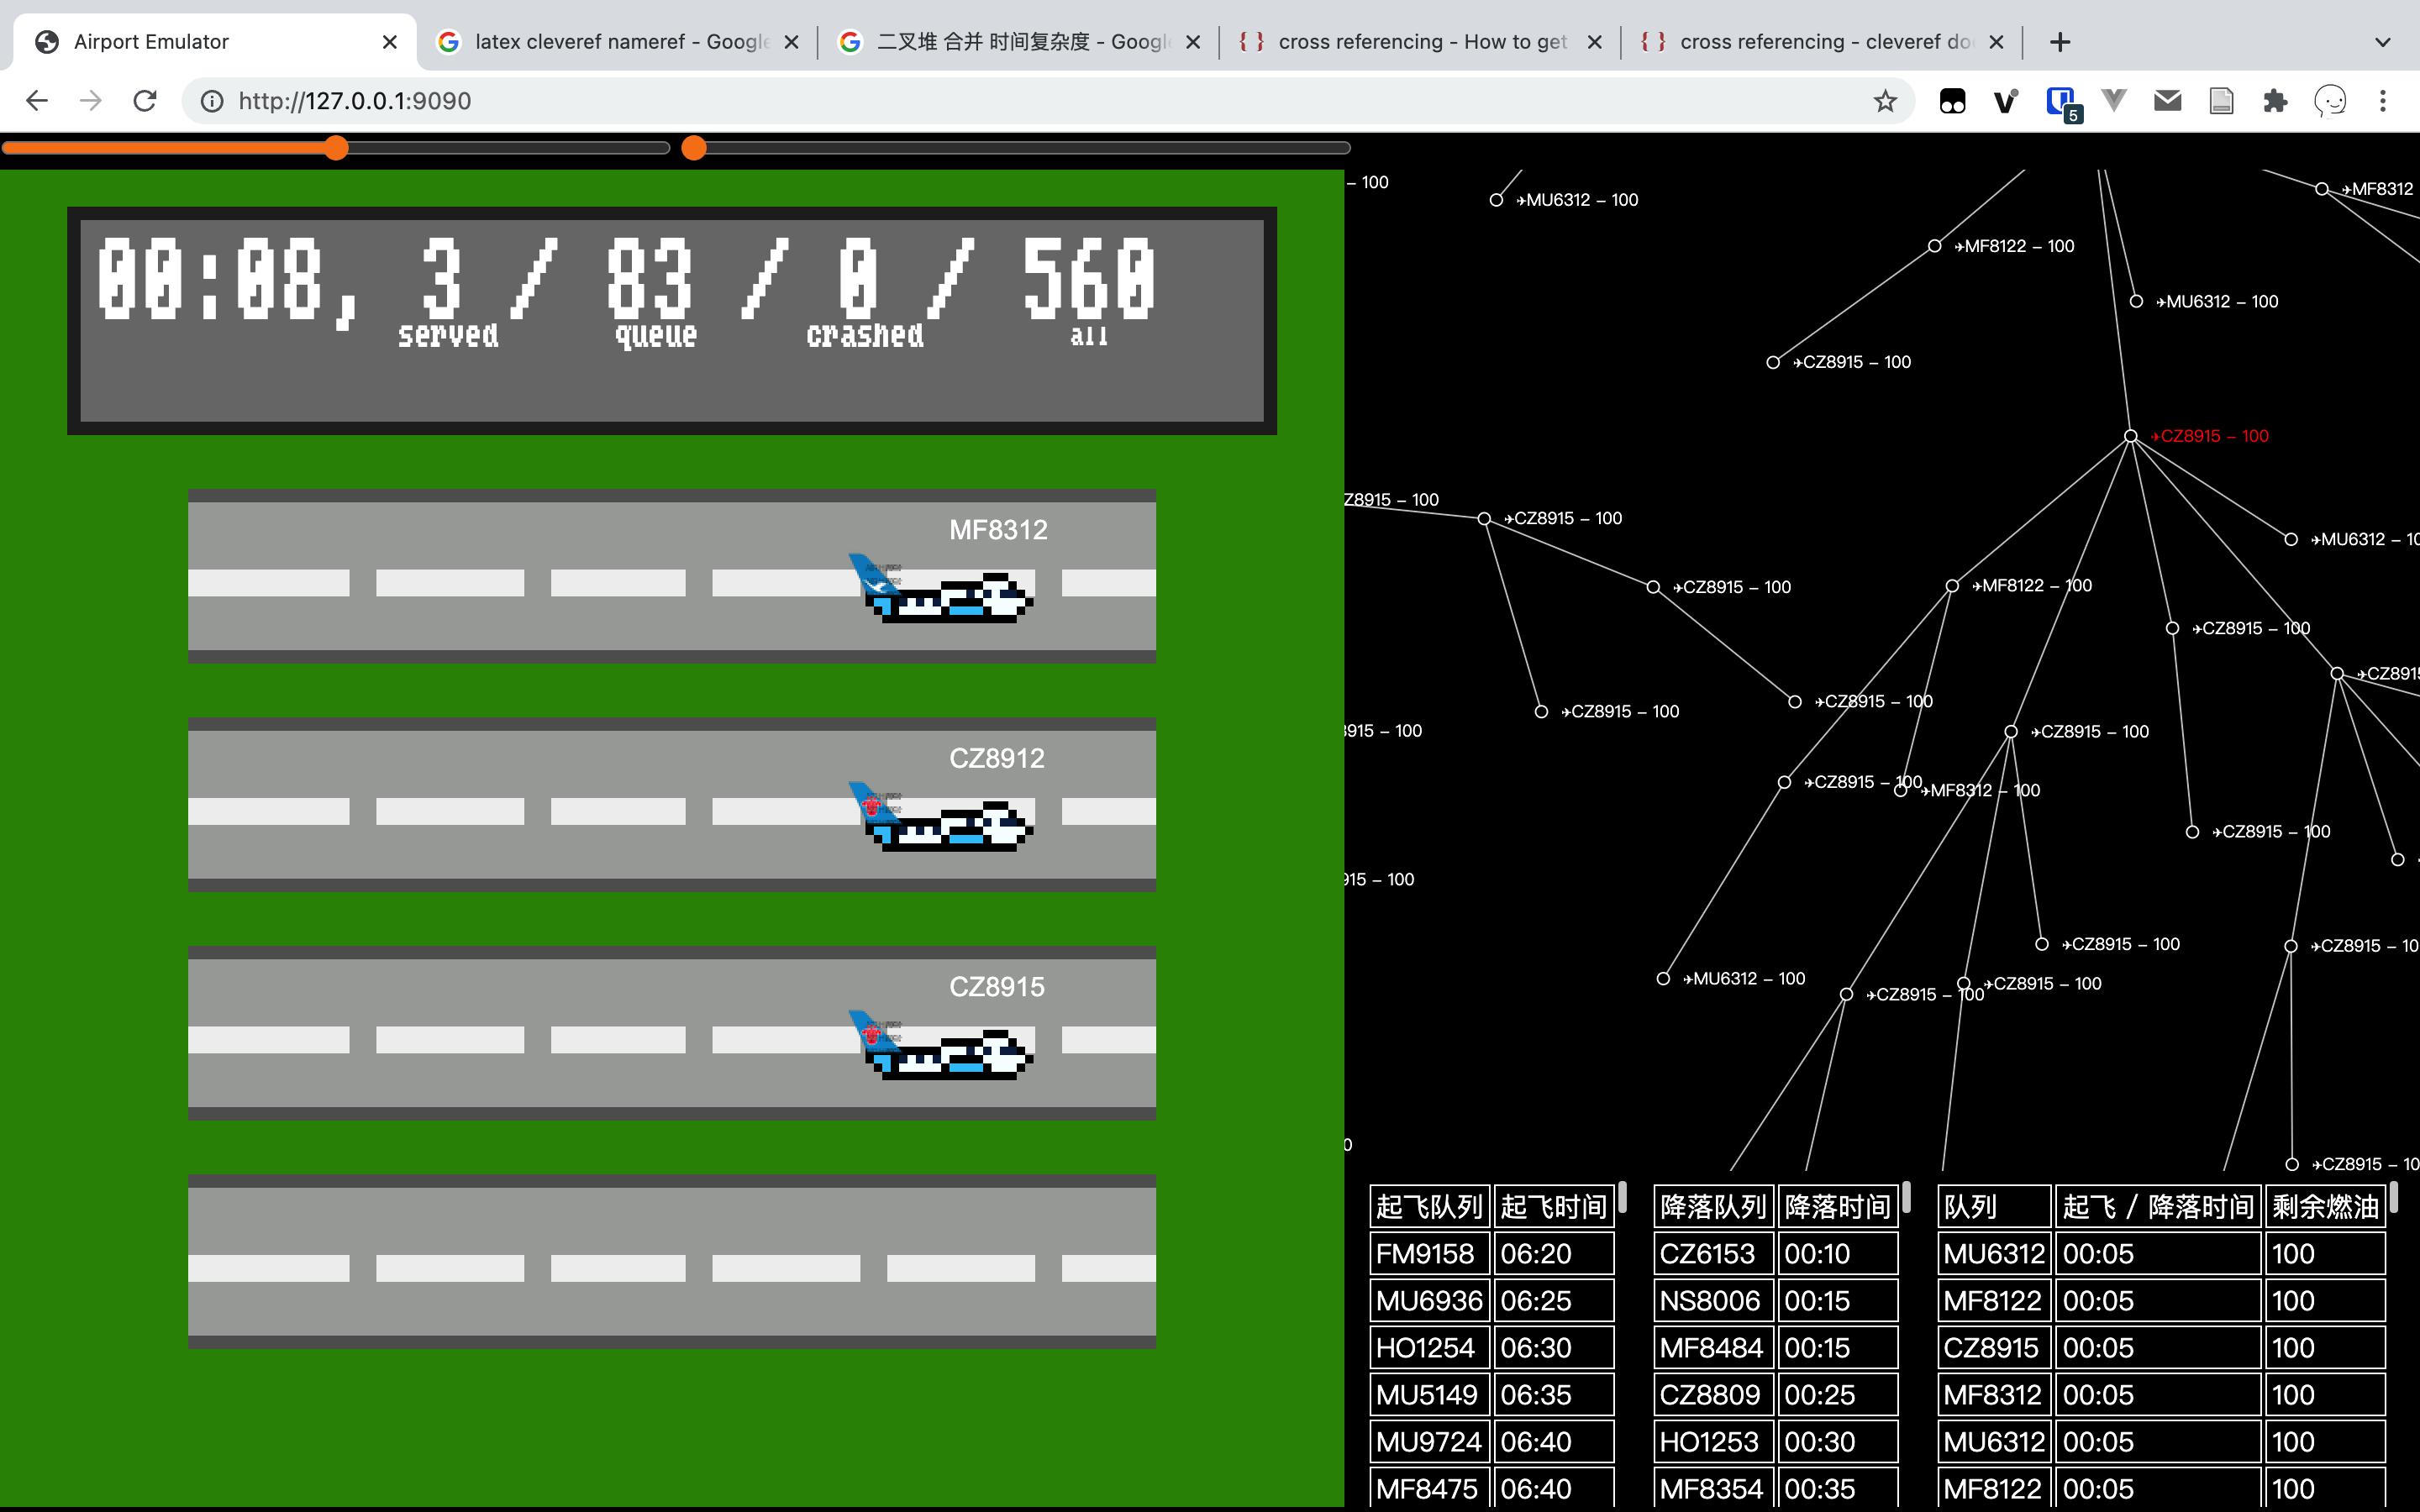
\includegraphics[width=0.9\textwidth]{images/test-crash-1}
    \caption{正常降落、记录燃油\quad 运行结果}
    \label{fig:test-crash-1}
\end{figure}

\begin{figure}[htp]
    \centering
    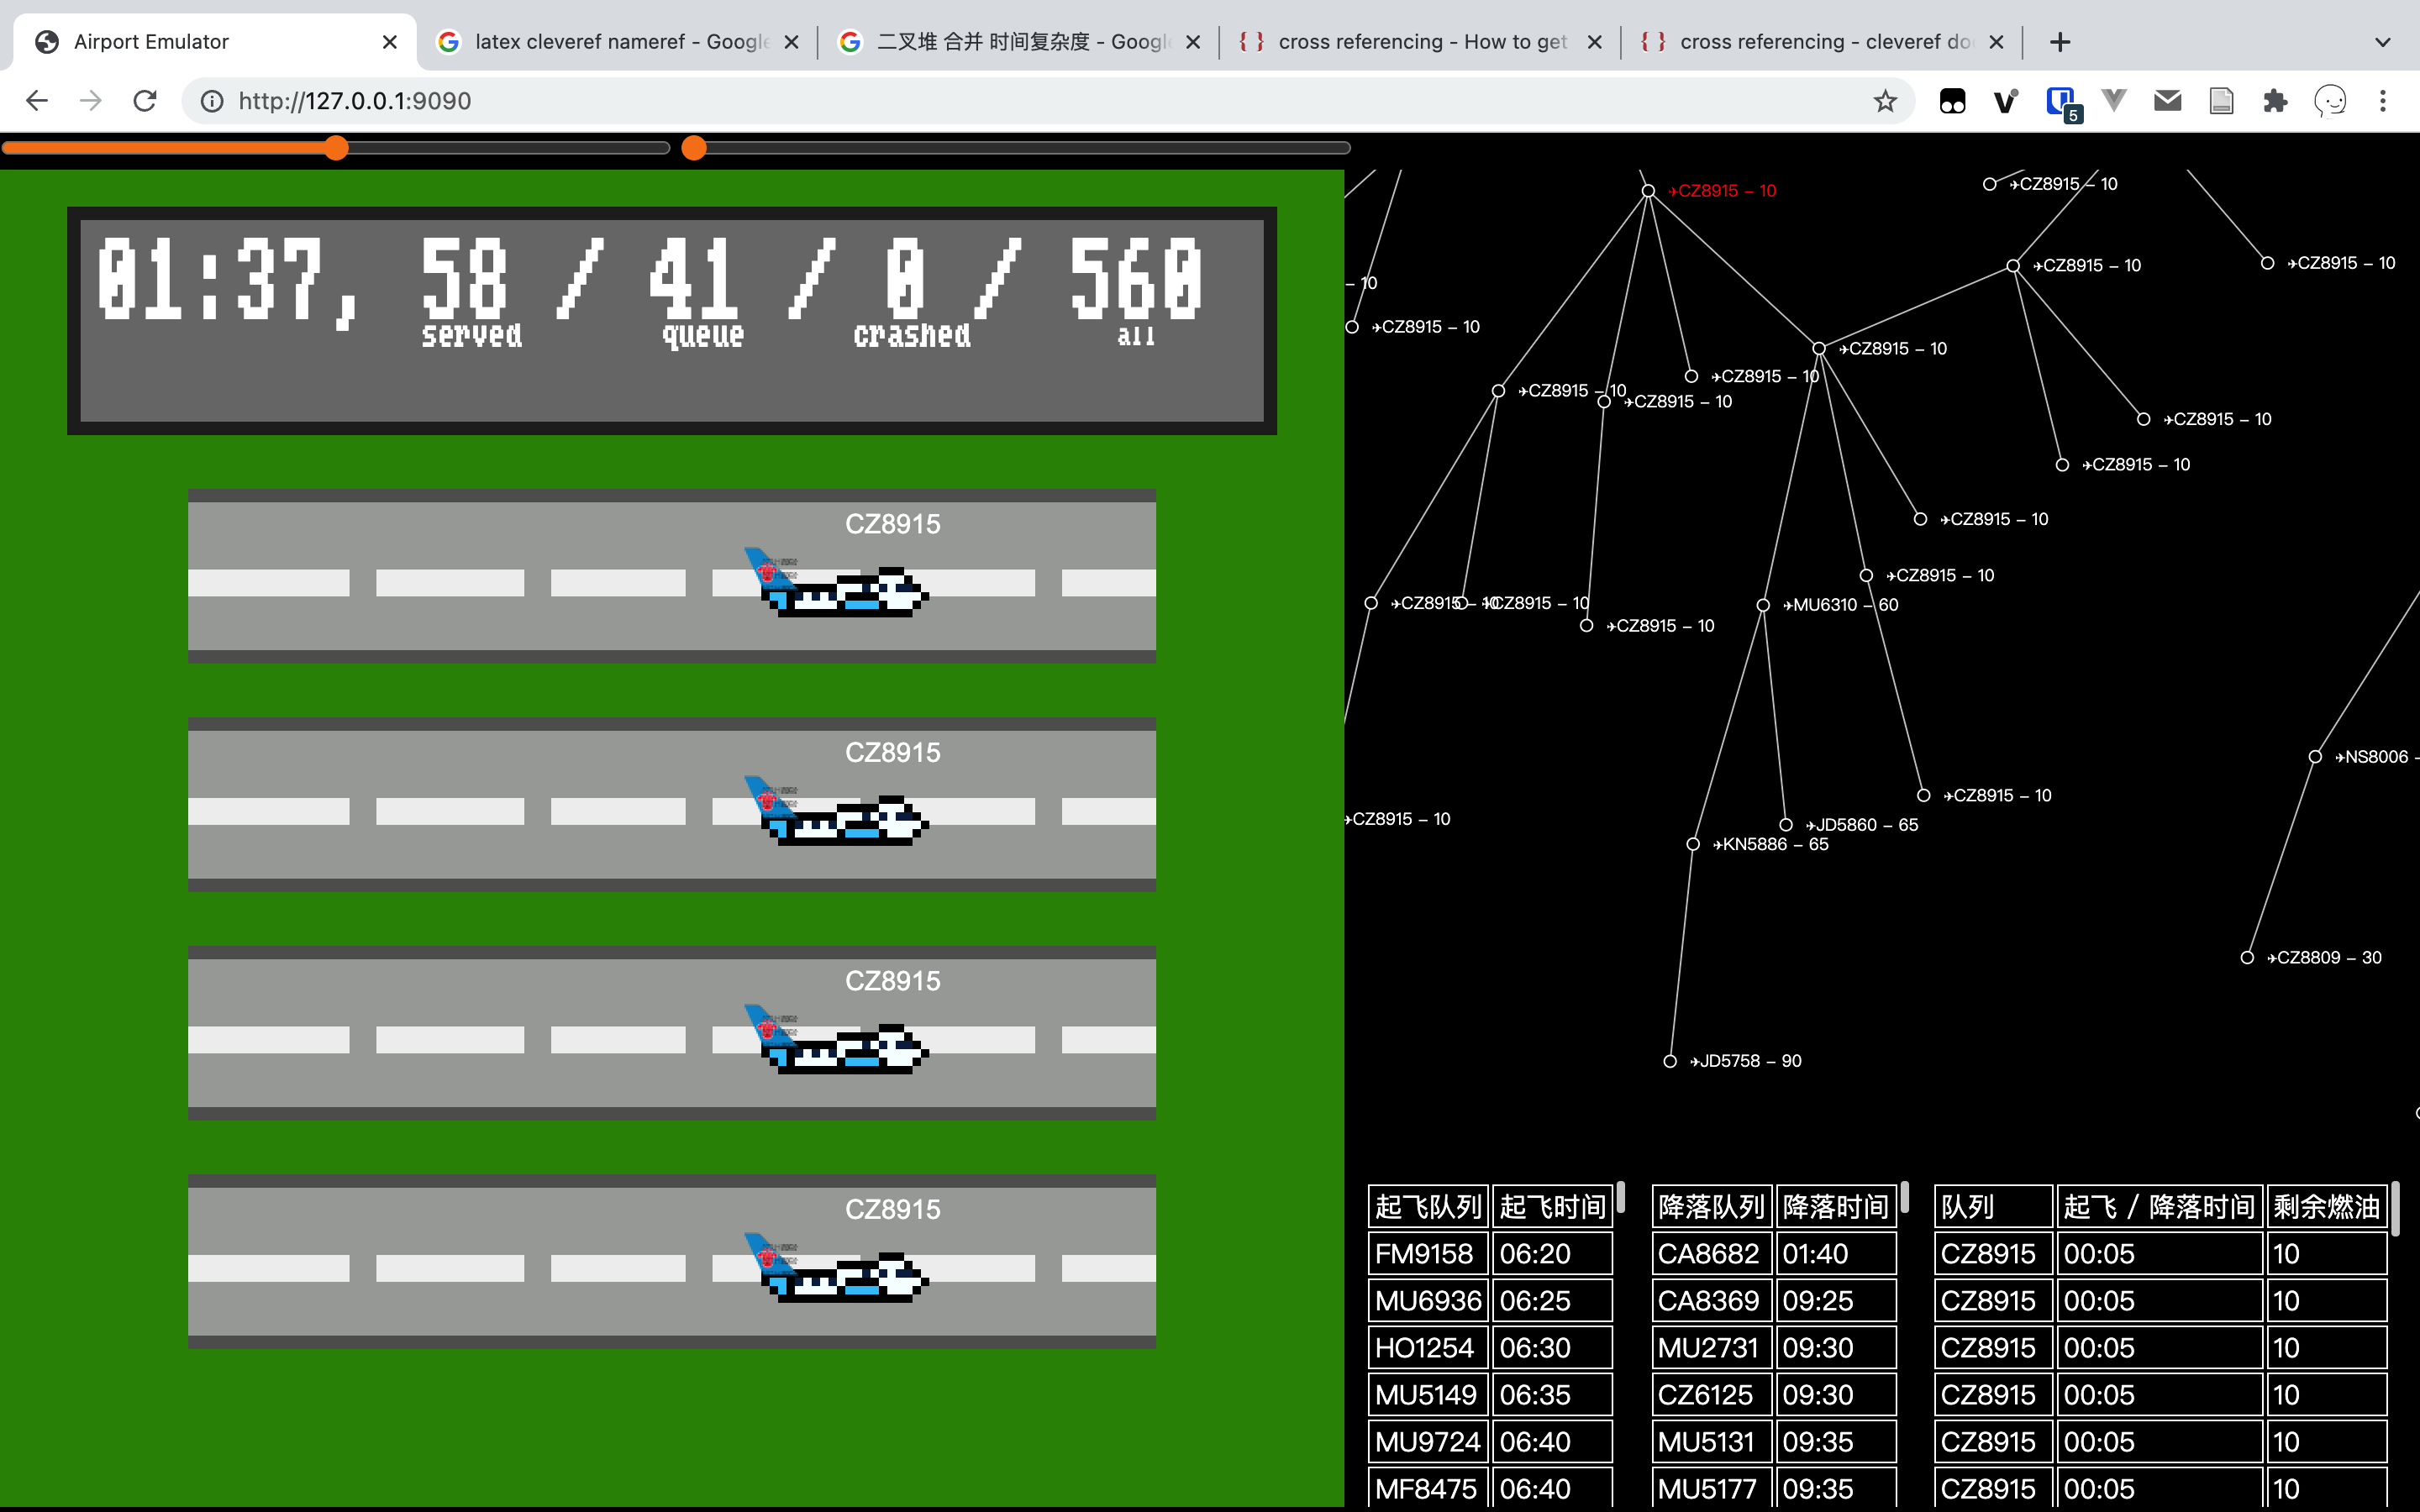
\includegraphics[width=0.9\textwidth]{images/test-crash-2}
    \caption{使用紧急降落跑道\quad 运行结果}
    \label{fig:test-crash-2}
\end{figure}

\begin{figure}[htp]
    \centering
    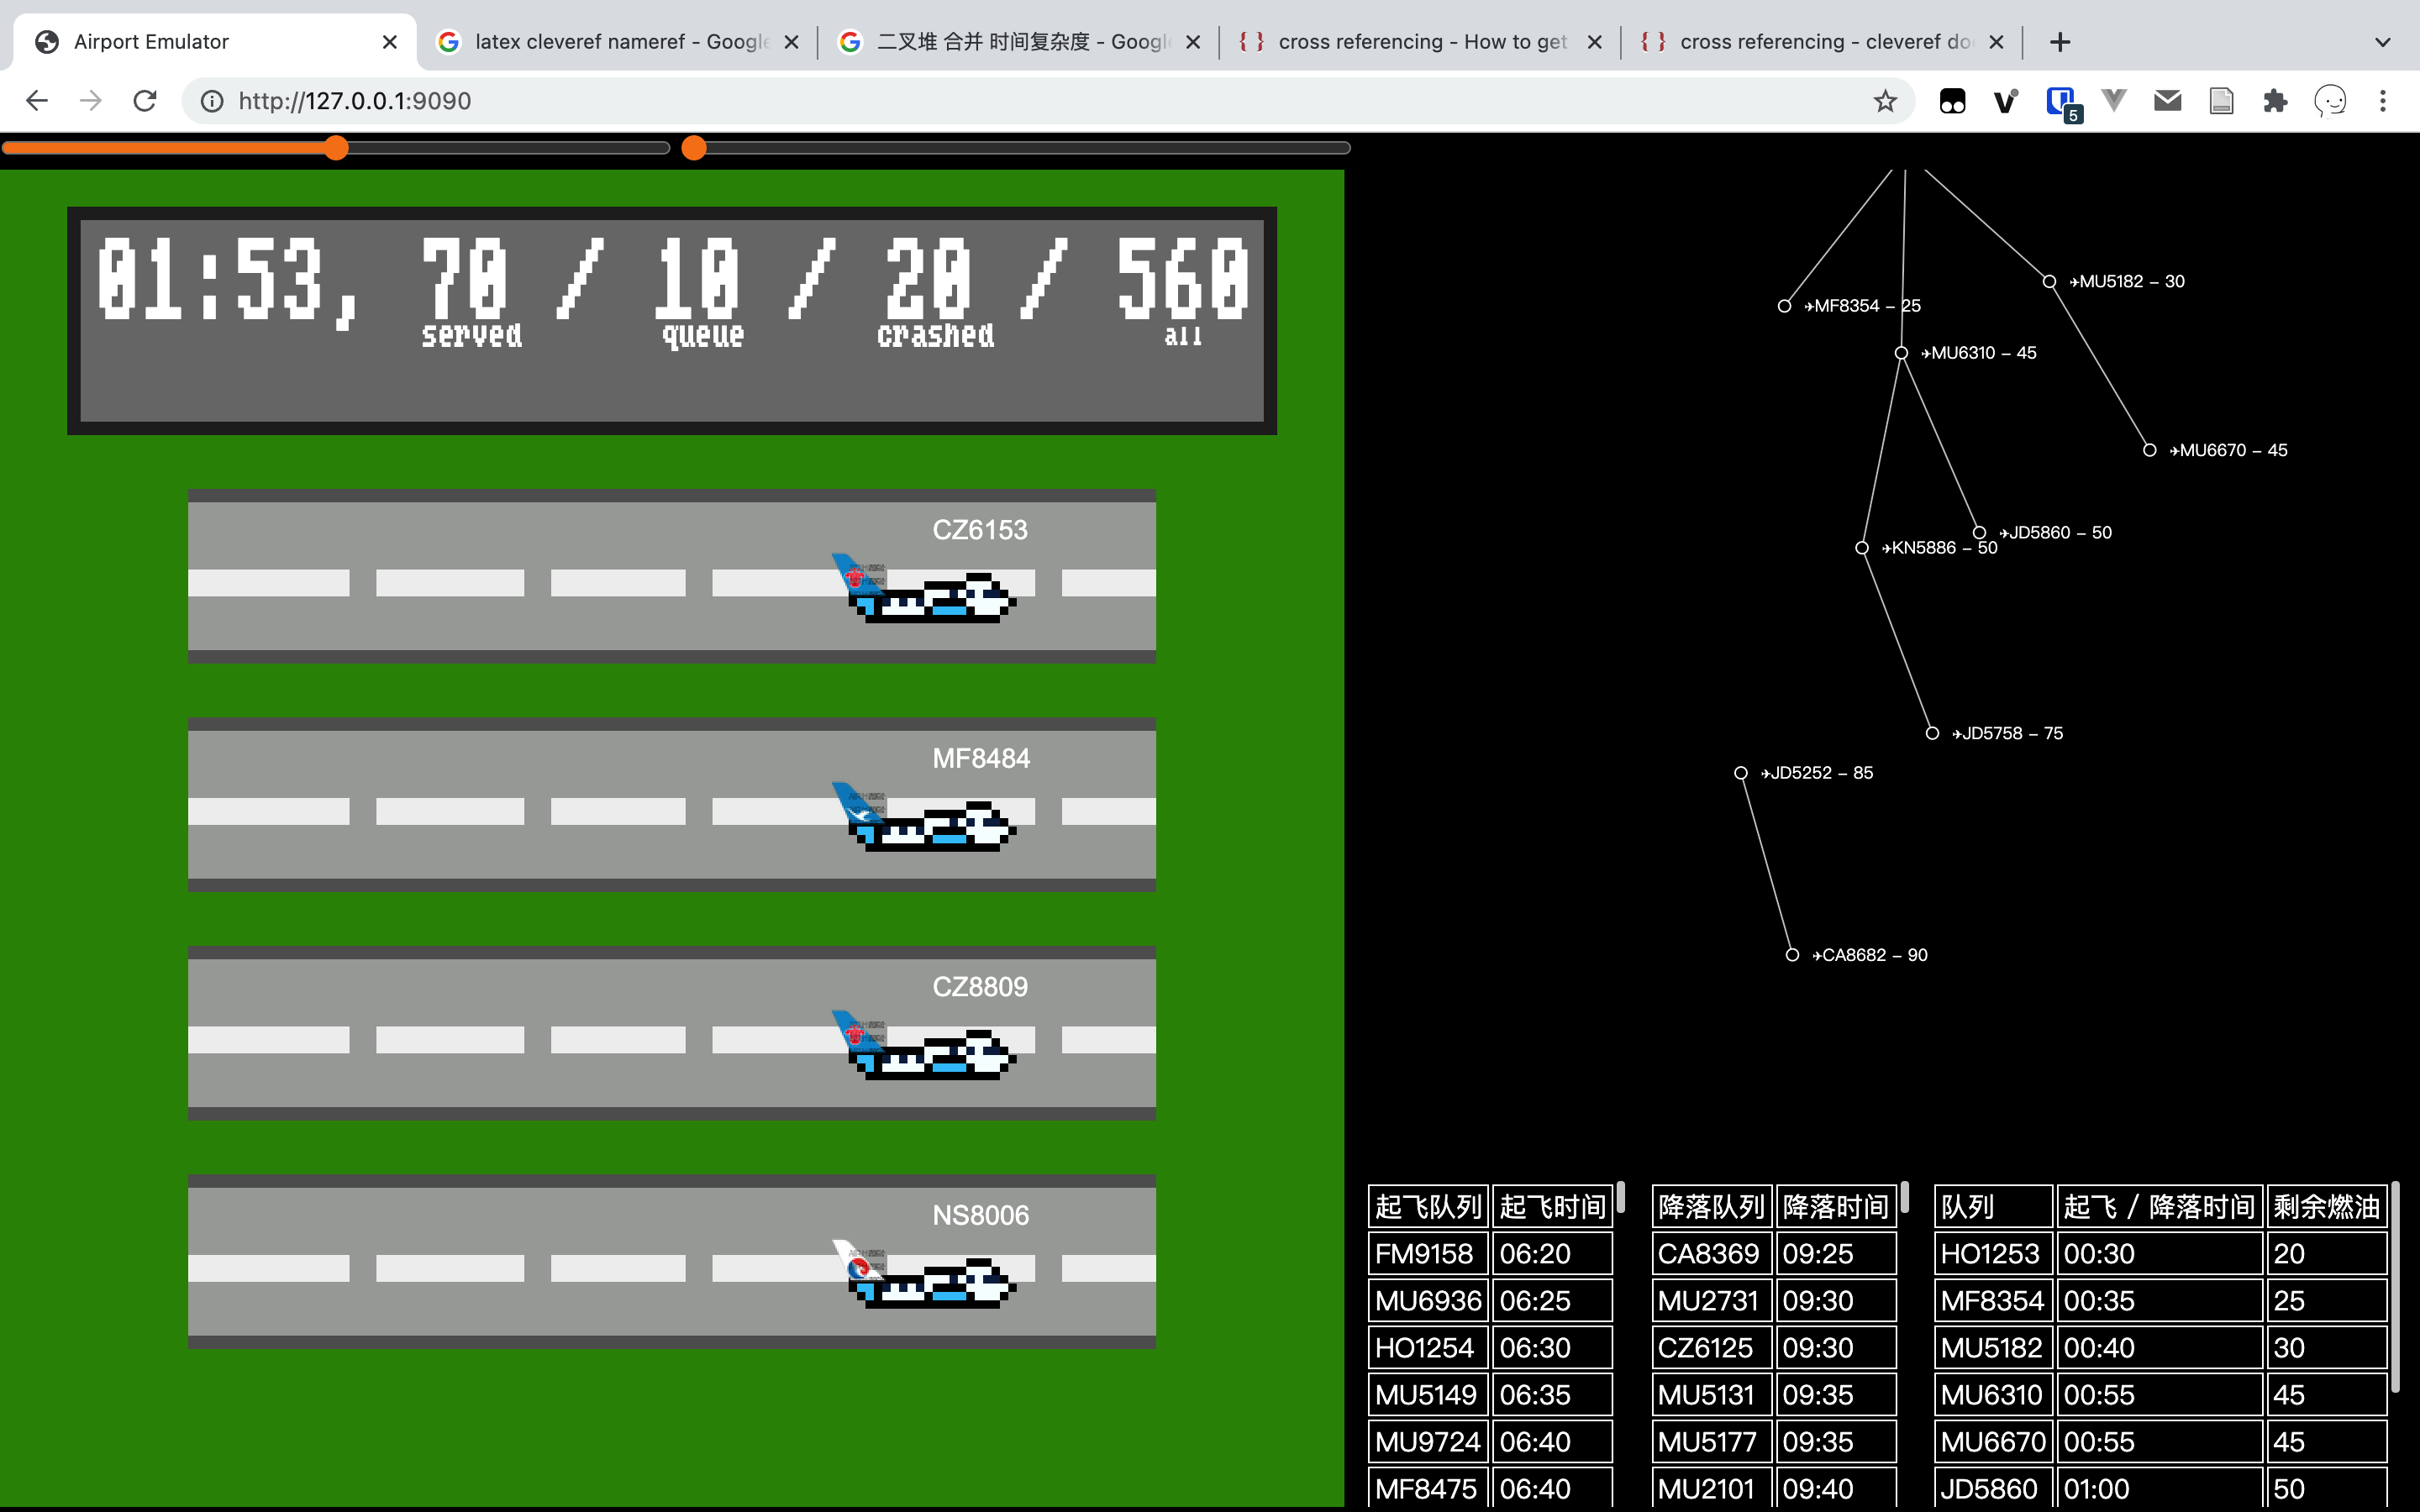
\includegraphics[width=0.9\textwidth]{images/test-crash-3}
    \caption{坠毁计数\quad 运行结果}
    \label{fig:test-crash-3}
\end{figure}

\section{总结与提高}
本项目具有以下特色:
\begin{outline}
    \1 创新性的使用『多级反馈队列』算法调度飞机
    \1 实现并应用了\fibheap , 在不提升时间复杂度的情况下实现动态优先级的计算与更新
    \1 实现了如下拓展功能:
        \2 飞机起飞、降落动画的渲染
        \2 飞机尾翼图标的动态渲染
        \2 逻辑帧与渲染帧分离的时钟速率系统
        \2 \fibheap 的可视化、力反馈图展示
\end{outline}

在实现项目的过程中,我也收获了许多。
\begin{outline}[enumerate]
    \1 在理解并实现\fibheap 的过程中,我加深了对于使用势函数分析算法的均摊复杂度的方法,并理解了\fibheap 的势函数的设计的原因。

        在之前分析简单算法的时间复杂度时,某一步的操作与下一步操作的时间没有关系,只需要分别分析每一步子问题的数量和子问题消耗的时间。但是,对于\fibheap 这样的复杂算法,每一步操作的时间都会影响下一步操作的时间。如:EXTRACT-MIN 时,我们首先将最小值的孩子放入根链表中,增加了整体的势,使得之后的操作变慢。接着,我们合并了根链表中度数相同的节点,使得其势显著减小。这样,整体来看,一次EXTRACT-MIN的时间复杂度仍为$O(\lg n)$。
    
    \1 在设计时钟速率功能的过程中,最开始我没有分离逻辑帧和渲染帧。这就导致了速率过快的时候,渲染速率较慢,成为系统最大的瓶颈。

        在调查了其他项目的实现后,我决定分离逻辑帧和渲染帧,也就是在一个渲染帧中执行多个逻辑帧。这样,系统的渲染速度就不再成为系统的瓶颈,时钟速率也可以设置更高的最大值。
    
    \1 在不同的应用场景下,对于同一个数据结构要采用不同的实现。如,在本项目中,由于有大量的DECREASE-KEY操作,选用\fibheap 可以加快整个系统的运行速度和时间复杂度。类似的,对于求图的最短路的 dijkstra 算法而言,每次松弛操作也有大量的DECREASE-KEY操作,如果选用\fibheap 就可以把时间复杂度从$O(n \lg m)$ 降低到$O(n \lg n)$。
\end{outline}

\bibliographystyle{gbt7714-numerical}
\bibliography{course-design-report}

\end{document}
